%Every piece of package I've acumulated over the last years
%%%%%%%%%%%%%%%%%%%%%%%%%%%%%%%%%%%%%%%%%%%%%%%%%%%%%%%%%%%%%%%%%%%%%%%%%%%%%%%%%%%%%%%%%%%%%%
\documentclass[a4paper,12pt]{article}
\usepackage[utf8]{inputenc}
\usepackage{imakeidx}
\usepackage{graphicx}
\usepackage{float}
\usepackage{amsmath}
\usepackage[backend=bibtex,style=verbose]{biblatex}
\bibliography{bibliography}
\usepackage{csquotes}
\usepackage{tcolorbox}
\usepackage{multirow}
\usepackage{caption}
\usepackage{afterpage}
\usepackage[margin=0.5in]{geometry}
%%%%%%%%%%%%%%%%%%%%%%%%%%%%%%%%%%%%%%%%%%%%%%%%%%%%%%%%%%%%%%%%%%%%%%%%%%%%%%%%%%%%%%%%%%%%%%
\begin{document}

\title{Practica 1: Simulaciones analógicas y técnicas numéricas}
\author{D'Andrade Furlanetto, Gabriel}
\maketitle

\section{Fundamento físico y objetivos}
Una enorme clase de problemas de electrostática no son más que resolver una PDE elíptica\footnote{De hecho, algunos autores afirman que la electrostática \textit{es} el estudio de la ecuación de Laplace, la más típica ecuación elíptica. Para una explicación detallada, \cite[111]{griffiths}}, o sea, que tienen solución determinada unicamente las condiciones de borde apropiada: Son un problema de Condiciones de Borde (BVP)\footnote{Para más información sobre el tema, \cite{pde}.}.

Cada uno de los problemas que trataremos van a ser diferentes condiciones de borde para la ecuación de Laplace:
$$\vec{\nabla}^2 \phi = 0 $$

Vamos a resolver el problema de dos maneras no-analíticas distintas: Primeramente, resolveremos un problema equivalente con corrientes estacionarias, después, utilizaremos técnicas numéricas estándar de elemento finito. 

Justificar formalmente que los problemas son equivalentes puede ser un poco complicado, pero para nosotros basta notar que es un material óhmico, o sea, que $\vec{E} = \sigma \vec{J}$, esto es, que las mismas condiciones de borde para el campo y la corriente producirán un mismo potencial salvo una constante multiplicativa.\footnote{Estas son condiciones de Neumann, o sea, sobre las derivadas del potencial en los bordes.} 

\section{Realización practica}

Para la primera parte de cada problema, utilizamos una trazadora analógica con el conmutador en $10V$ y lo conectamos a los electrodos del panel del problema. Después de comprobar que el montaje está bien hecho, utilizamos el potenciómetro y la empezamos a trazar curvas equipotenciales para los valores separados por $1V$ ($0V, 1V, \ldots 10 V$)

Para la segunda, utilizamos el Software QuickView para resolver el problema numéricamente. El programa utiliza métodos bastante típicos de elementos finitos, que subdividen nuestro espacio en \textit{meshes} y calculan la diferencia finita (no la derivada) en cada punto, de manera que se verifiquen las condiciones de borde.
\pagebreak

\subsection{Problema 1}


\begin{figure}[h!]
\centering
	\caption{Fotografía del problema a resolver}
	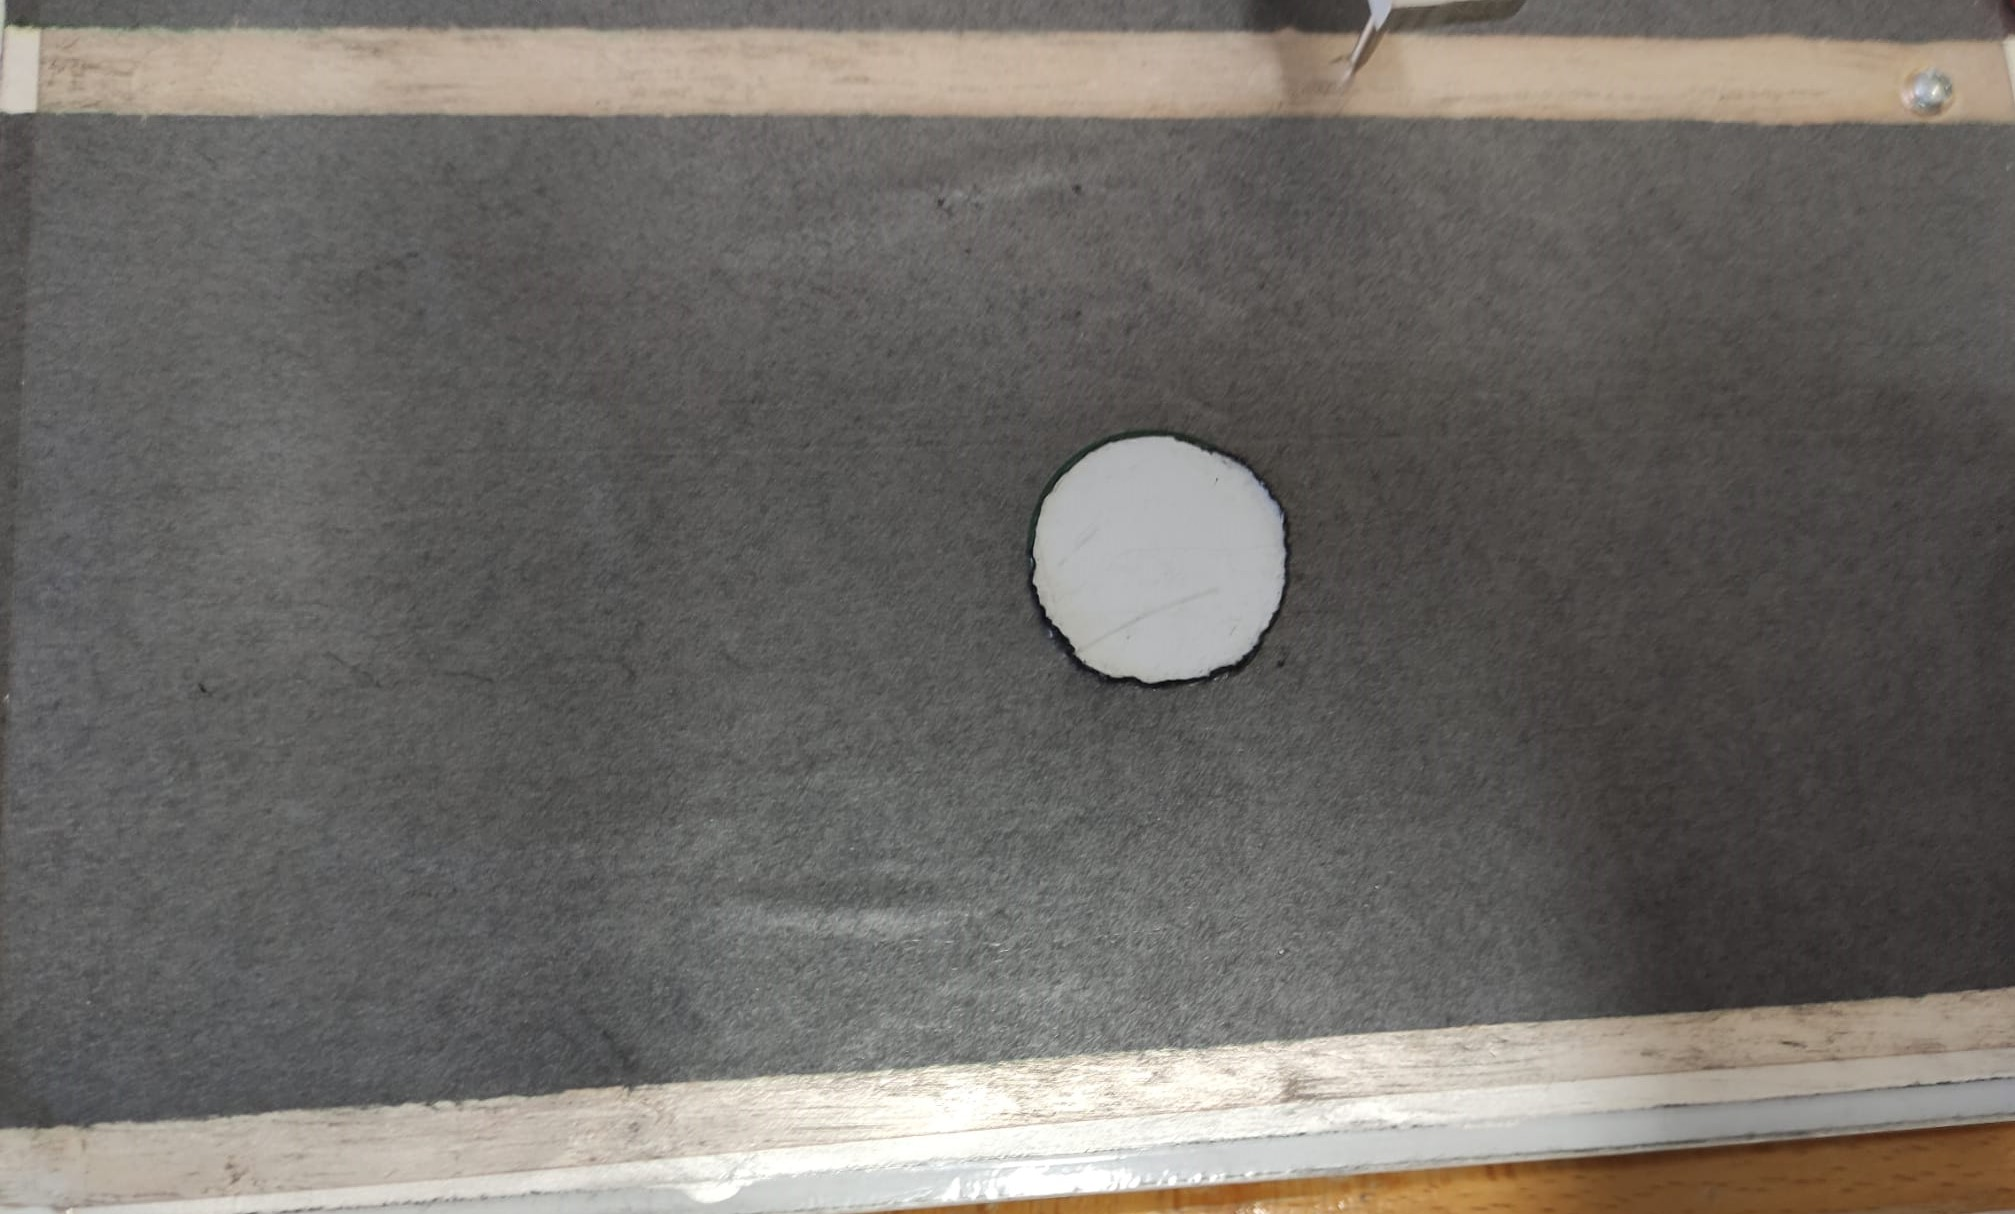
\includegraphics[width=0.5\textwidth]{Prob1pic.jpeg}
\end{figure}
Físicamente, esto corresponde aproximadamente al problema del conductor esférico en un campo eléctrico uniforme, si se deprecian los efectos de borde de las placas paralelas que generan este condensador. Trazando las equipotenciales, tenemos la siguiente figura:
\begin{figure}[h!]
\centering
	\caption{Fotografía de las equipotenciales}
	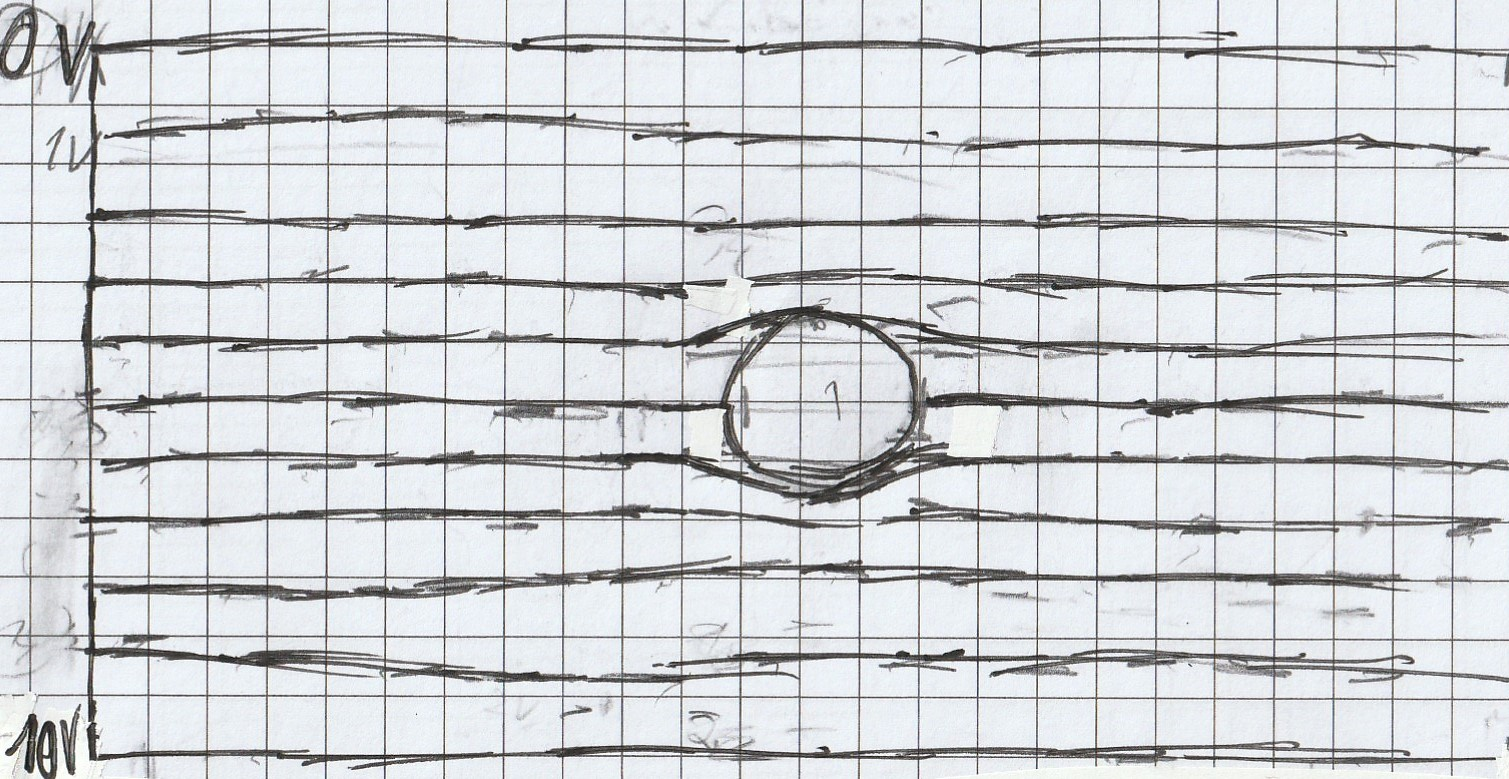
\includegraphics[width=0.5\textwidth]{problem1equi.jpg}
\end{figure}

Finalmente, tenemos la solución numérica:

\begin{figure}[h!]
\centering
	\caption{Simulación del problema mediante QuickField}
	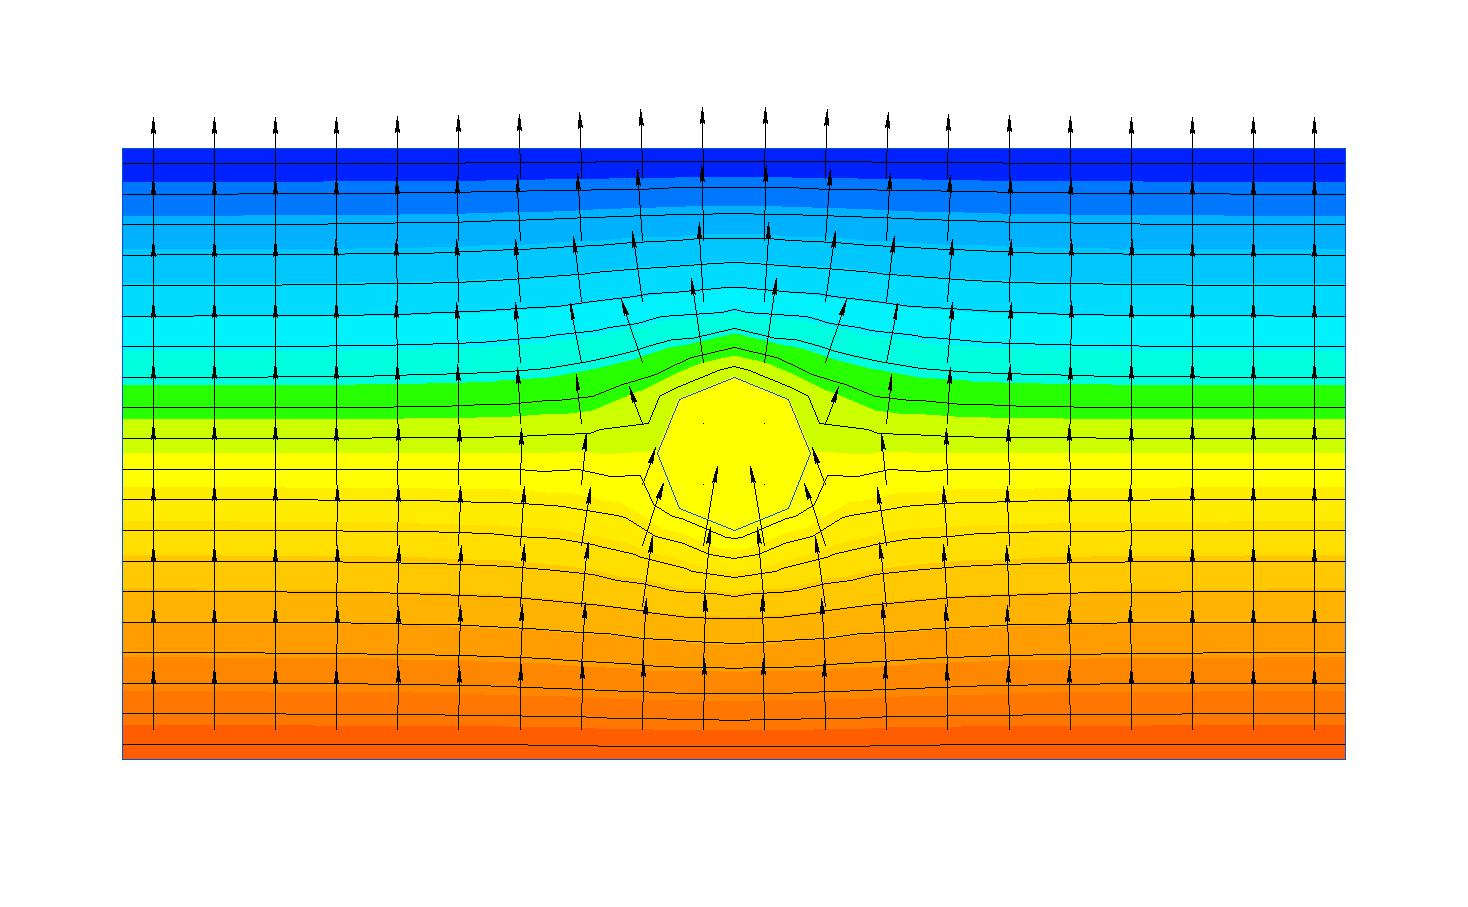
\includegraphics[width=0.7\textwidth]{test1.jpg}
\end{figure}

\pagebreak 
\subsection{Problema 2}
\begin{figure}[h!]
\centering
	\caption{Fotografía del problema a resolver}
	\includegraphics[width=0.5\textwidth]{Prob2pic.jpeg}
\end{figure}
Físicamente, esto corresponde aproximadamente al problema de las placas plano-paralelas con un punto (que no está en el centro) a potencial constante (en este caso, a $0V$). Este, bastante más que el primer problema, es bastante complicado de resolver analíticamente y ilustra la importancia que tienen los métodos no-analíticos para poder hablar del problema.
\begin{figure}[h!]
\centering
	\caption{Fotografía de las equipotenciales}
	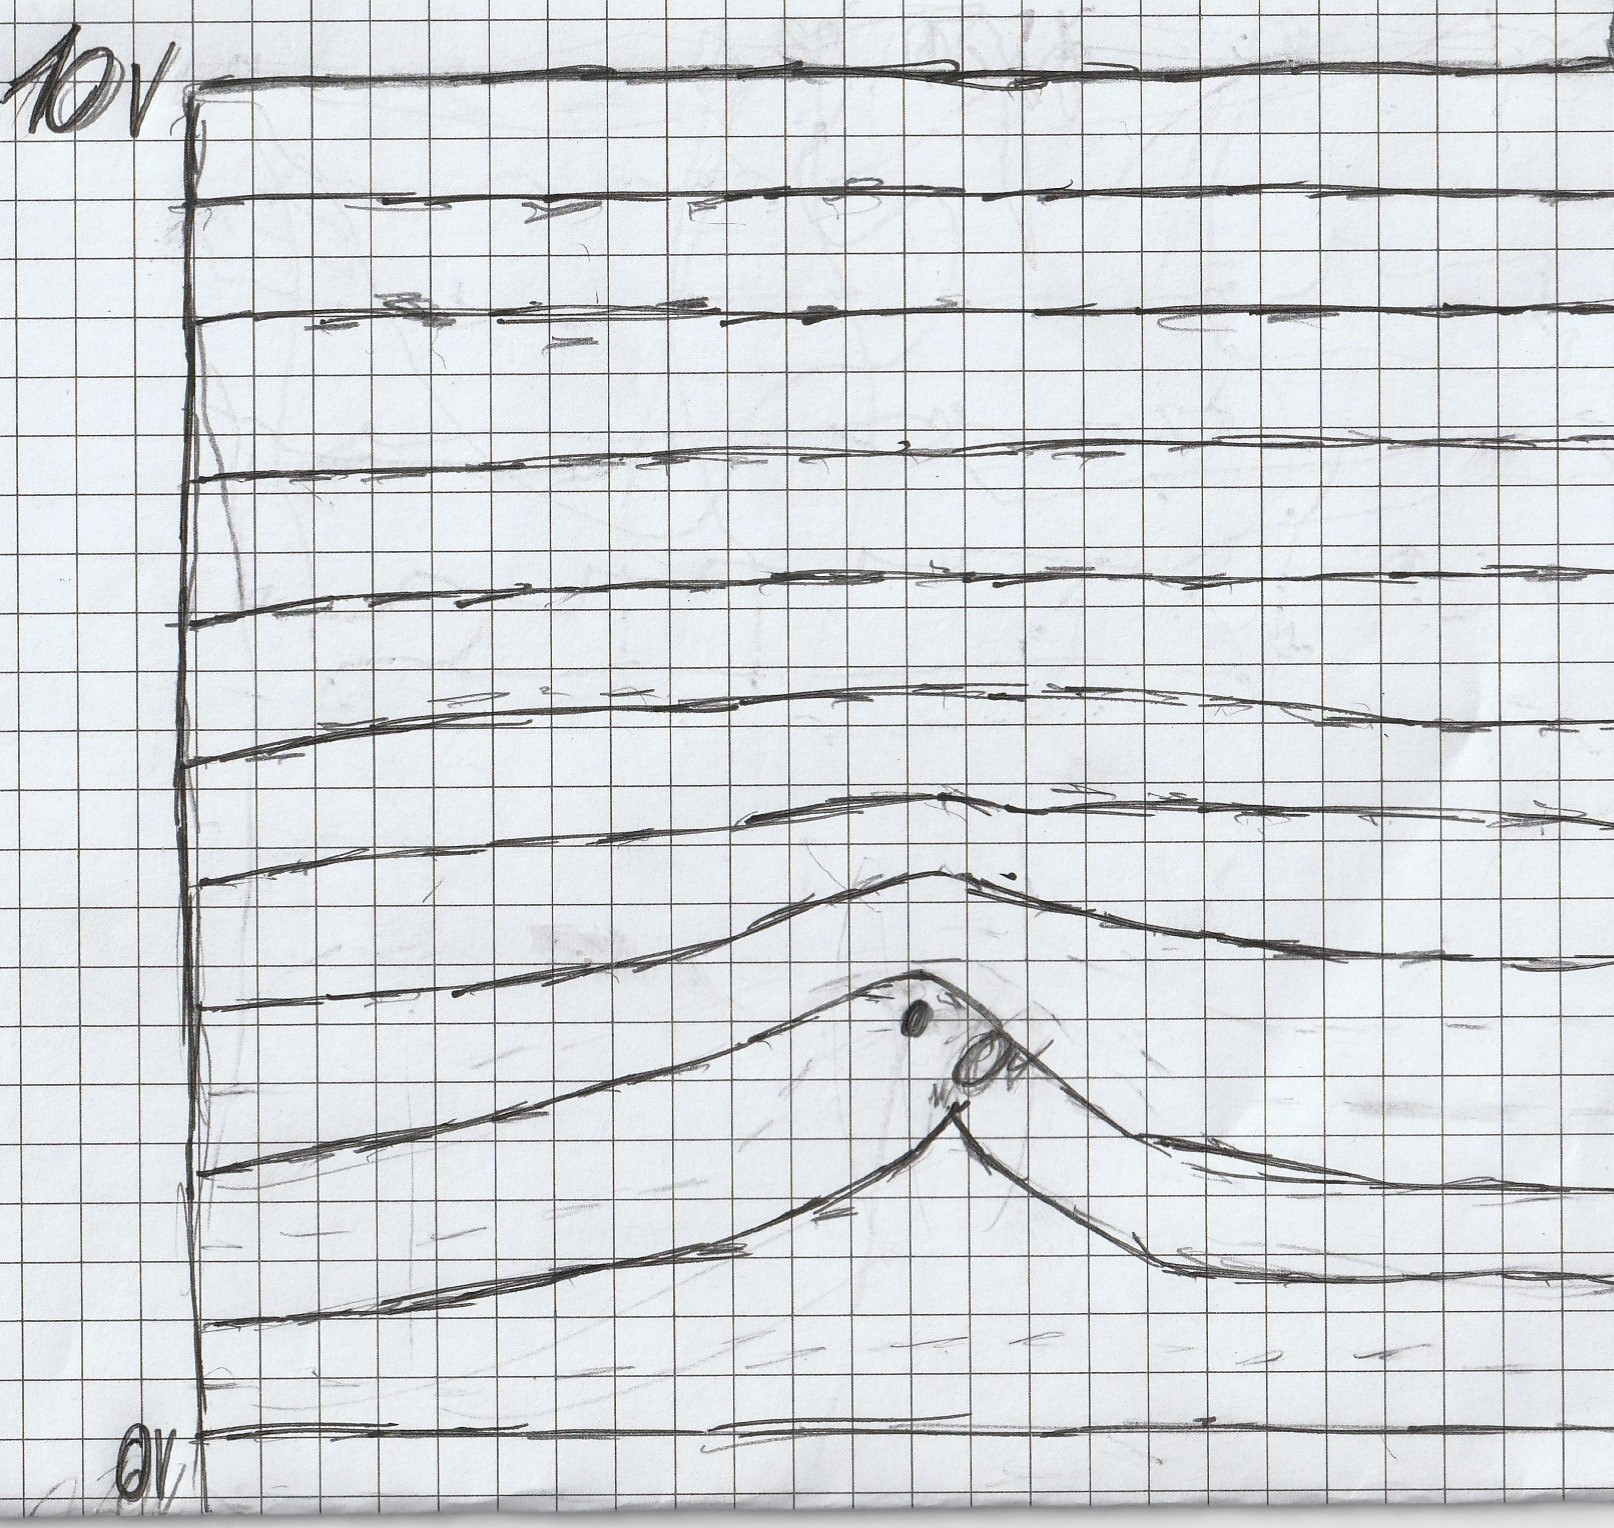
\includegraphics[width=0.5\textwidth]{problem2equi.jpg}
\end{figure}

Finalmente, tenemos la solución numérica:

\begin{figure}[H]
\centering
	\caption{Simulación del problema mediante QuickField}
	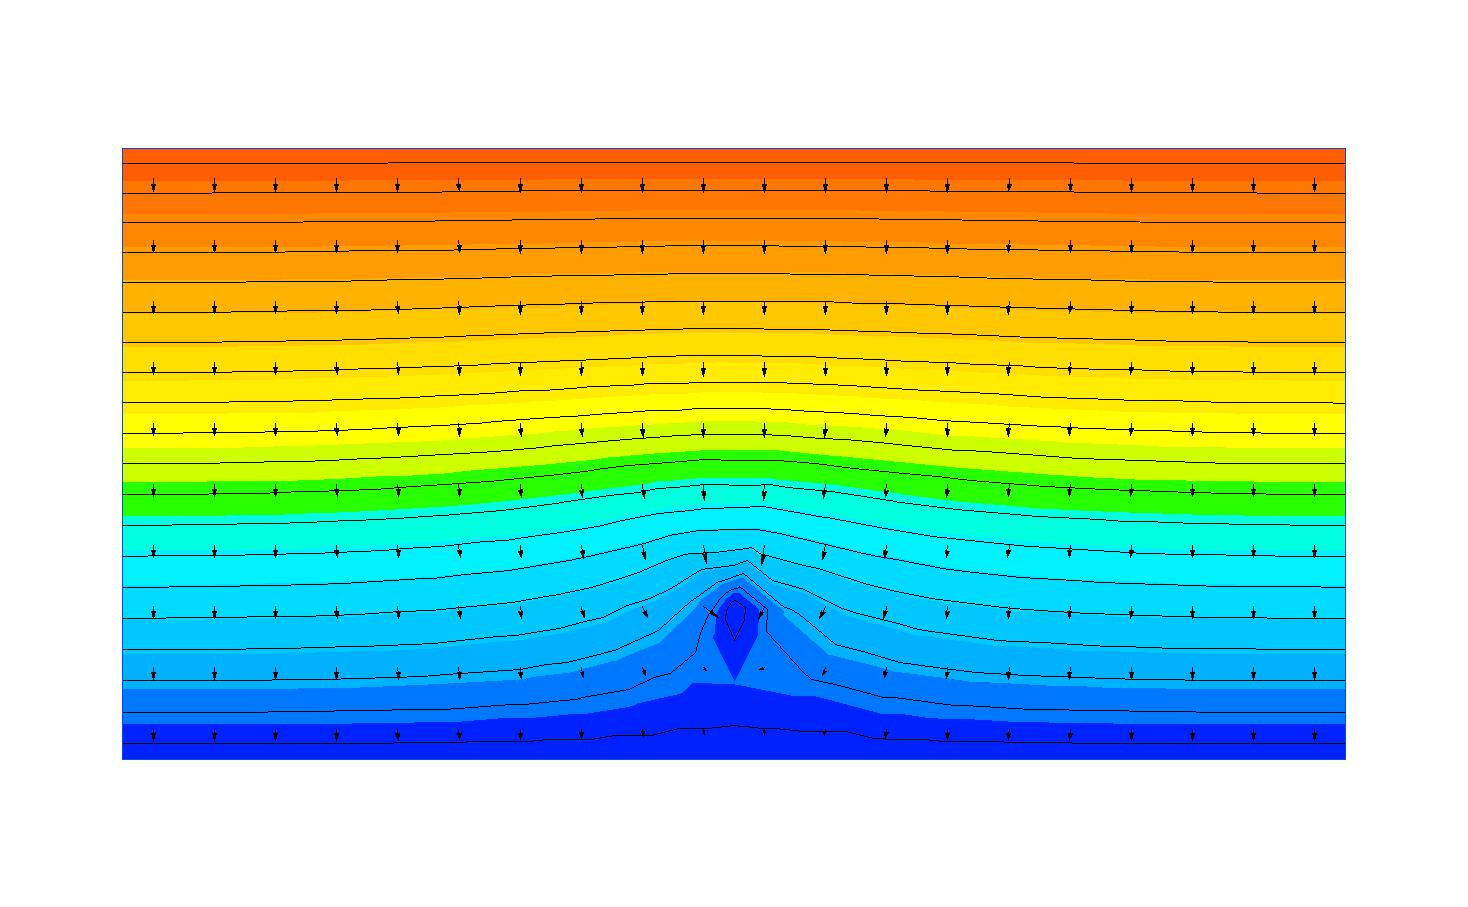
\includegraphics[width=1\textwidth]{problem 2.jpg}
\end{figure}


\section{Comentarios}

La utilidad de estos métodos no está en resolver problemas como el primero, que tienen solución analítica bastante estudiada, pero para problemas como el segundo, donde encontrar una solución analítica es extremadamente difícil o directamente imposible pero estudiar \textit{alguna} solución es interesante por si mismo, estos métodos nos proporcionan una forma sistemática de hacerlo. $$\frac{D \dot{q_{j}}}{Dt}= Q_j$$
\printbibliography
\end{document}

